% !TeX program = xelatex
% Compile from the repository root. In Overleaf, select XeLaTeX and this main file.
% The figure directory below also supports a flat upload of the five figure PDFs.
\documentclass[aps,prd,12pt,twocolumn,superscriptaddress,floatfix]{revtex4-2}

% REVTeX 4.2 needs the legacy array interface on recent TeX Live releases.
\usepackage{array}[=2016-10-06]
\usepackage{kotex}
\usepackage{amsmath}
\usepackage{booktabs,tabularx}
\usepackage{graphicx}
\usepackage[a4paper,margin=0.7in]{geometry}
\usepackage{xurl}
\usepackage[hidelinks]{hyperref}
\graphicspath{{artifacts/figures/d7_paper_evidence/20261117_final/}{./}}
\setlength{\emergencystretch}{2em}
\raggedbottom

\begin{document}

\title{Candidate Quality and Logical-Transition Selection in Neural Pre-Decoding for Surface Codes}
\author{Jaemin Jeon}
\affiliation{Korea University}
\date{November 18, 2026}

\begin{abstract}

본 연구에서는 surface code의 detector bit를 국소적으로 수정하고, 같은 shot에서 수정 전후의 PyMatching 논리 예측을 비교했다. 거리 7의 강한 ZZ 잡음에서 top-1 후보는 원본 오답 10,501쌍을 고쳤고 원본 정답 25,126쌍을 해쳤다. 수정할 shot을 고정한 oracle이 top-1보다 추가로 맞힌 25,131쌍 중 25,126쌍은 원본 정답을 보존한 경우였다. 독립 맵에서 shot별 margin의 정확도 차이는 원본 대비 \ensuremath{-}0.035 pp(97.5\% 구간 [\ensuremath{-}0.082, +0.013] pp)였다. 후속 대조 실험에서는 같은 후보 예산에서 학습 방식이 비학습 국소 열거보다 원본 오답에 정답 후보를 +11.07 pp 더 자주 제공했다(95\% 구간 [+7.63, +14.51] pp). 후보 생성 전 게이트는 별도의 새 맵 24개에서 기존 후단의 512-shot 배치 시간을 평균 119 ms 줄였고, 원본 PyMatching 대비 정확도 차이는 +0.028 pp로 불확실했다. 후속 실험에서는 데이터 큐비트 단일 큐비트 채널의 총 오류 확률을 유지하며 Pauli 편향을 바꾸고, 해당 편향을 반영한 PyMatching을 기준선으로 사용했다. 편향 \(\eta=p_Z/(p_X+p_Y)=20\)의 독립 평가에서 기존 margin의 추가 이득은 +0.004 pp(95\% 구간 [\ensuremath{-}0.086, +0.094] pp)였다. 후보 CNN을 고정하고 편향 자료로 4-class 채택 모델을 새로 학습한 뒤 별도의 독립 맵에서 평가한 이득도 +0.018 pp(95\% 구간 [\ensuremath{-}0.070, +0.107] pp)였다. 이들 최종 독립 주 비교에서 추가 정확도 이득은 확인되지 않았다.

\textbf{주제어} surface code, 양자 오류 정정, 사전 디코더, PyMatching, 논리 전이

\end{abstract}

\maketitle

\section{서론}

Surface code는 국소 stabilizer를 반복 측정해 오류에 대한 정보를 얻는다 \cite{fowler2012}. 측정 기록에서 추출한 detector event는 어떤 검사가 기대한 값에서 벗어났는지 나타낸다. 디코더는 이 사건들과 양립하는 오류 경로를 추정해 논리 관측량의 반전을 예측한다. 본 연구의 기준 디코더는 그래프의 가중치로 최소 가중치 완전 매칭(MWPM)을 계산하는 PyMatching이다 \cite{higgott2022,sparseblossom2025}.

한 shot의 detector bit를 몇 개 뒤집은 뒤 다시 디코딩하면 원본 PyMatching이 틀린 논리 예측을 고칠 수 있다. 반대로 원본 예측이 맞는 경우에도 수정으로 논리 클래스가 바뀔 수 있다. 따라서 좋은 수정 후보를 생성하는 문제와, 실제 추론에서 어떤 후보를 선택할지 판단하는 문제를 구분해야 한다. 이 연구에서는 같은 shot에 원본과 수정 경로를 모두 적용해 두 판단의 차이를 측정했다. 또한 참값을 사용하는 oracle로 후보 집합이 허용하는 회복 범위를 구해, 후보 부족과 선택 손실을 구분했다.

기존의 국소 사전 디코딩 연구는 반복 측정에서 물리 오류를 국소적으로 처리한 뒤 잔여 syndrome을 전역 디코더에 전달하는 구조를 제시했다 \cite{chamberland2026}. 본 연구의 국소 수정은 시뮬레이션에서 detector bit에 적용하는 가설이다. 수정 전후에 동일한 후단 디코더를 두고 논리 예측을 비교하는 데 사용했다. 잡음 prior의 적합성을 분석한 Darmawan의 연구는 단일 큐비트 잡음 설정에서 디코더에 제공하는 모델을 바꿔 효과를 측정했다 \cite{darmawan2024}. 본 연구에서는 생성할 때 사용한 잡음과 매칭 그래프를 구성할 때 사용한 잡음을 교차시켜, 같은 수정의 효과와 선택을 다시 했을 때의 효과를 나눠 평가한다.

후보 선택에 확신도 정보를 넣는 방법도 비교했다. Gidney 등은 동일 syndrome에서 가능한 논리 결과에 따라 matching 비용이 달라지는 정도를 활용했다 \cite{yoked2025}. Decoder switching은 비용이 다른 두 디코더 사이에서 확신도를 기준으로 경로를 바꾼다 \cite{toshio2025}. 또한 디코더가 가정한 잡음과 실제 잡음이 다르면 논리 gap을 그대로 정답 확률로 해석하기 어렵다 \cite{hoyt2026}. 이에 본 연구는 같은 syndrome에서 계산한 클래스별 비용 차이가 detector 특징에 추가로 정보를 주는지, 원본 syndrome만으로 논리 전환을 판단하는 더 단순한 경로와도 비교했다.

ZZ 계수 비교에서는 총 오류량도 달라졌다. 후속 실험에서는 각 데이터 큐비트 단일 큐비트 채널의 총 오류 확률을 고정하고 X, Y, Z의 비중을 바꿨다. 실제 편향 회로에서 얻은 DEM으로 PyMatching 가중치를 구성한 뒤, 고정 후보 생성기와 기존 margin을 붙이는 효과 및 편향 자료로 채택 모델을 새로 학습하는 효과를 각각 새 맵에서 평가했다.

\section{사전 디코더와 비교 정책}

\subsection{회로와 논리 관측량}

Stim \cite{stim2021}으로 rotated surface code의 Bell-pair Z readout 회로를 샘플링했다. 주 실험은 거리와 syndrome 측정 라운드가 각각 7인 회로에서 수행했다. 각 shot의 참값은 두 관측량의 반전 비트 (z, x)다. 출력 순서는 [Z flip, X flip]이며, 클래스는 \(2z + x\)로 표현한다. 두 비트를 모두 맞힌 경우만 정답으로 계산했다. 이 지표의 논리 오류율은 한 비트라도 틀린 shot의 비율이다.

로컬 잡음 맵은 회로 위치별 물리 오류 확률을 정한다. 물리 오류율의 기준값을 0.0015로 두고, 각 맵에서 ZZ 계수가 0.05인 약한 조건 \(G_0\)와 0.25인 강한 조건 \(G_1\)을 구성했다. 두 조건은 로컬 맵과 이상 회로를 공유하며 서로 다른 sampler seed를 사용했다. 기본 잡음 및 swap 항은 고정했다. ZZ 계수를 높이면서 전체 오류량도 달라진다. \(D_0\), \(D_1\)은 각각 \(G_0\), \(G_1\)에서 얻은 detector error model(DEM)이다. 각 조건에 일반 MWPM과 correlated PyMatching을 적용했다.

Pauli 편향 실험은 같은 rotated 회로에서 ZZ 계수 0.05, swap 계수 0.02를 사용했다. 데이터 큐비트에 적용되는 단일 큐비트 gate와 idle의 DEPOLARIZE1 채널을 다음 확률로 구성했다.
\begin{equation}
\begin{aligned}
\eta&=\frac{p_Z}{p_X+p_Y},\\
p_X=p_Y&=\frac{q}{2(1+\eta)},\\
p_Z&=\frac{q\eta}{1+\eta}.
\end{aligned}
\label{eq:data-pauli-bias}
\end{equation}
여기서 \(q=p_X+p_Y+p_Z\)는 해당 위치의 기존 총 오류 확률이다. \(\eta=0.5\)에서 기존 균등 단일 큐비트 채널을 사용했고, 5와 20에서 Z 비중을 높였다. 측정·리셋 오류, ancilla의 단일 큐비트 잡음, 2-qubit depolarizing noise와 기존 ZZ·swap 항에는 같은 로컬 맵의 기존 확률을 사용했다. 따라서 \(\eta\)는 변경 대상인 데이터 큐비트 단일 큐비트 채널의 편향을 뜻한다. 회로 전체의 Pauli 오류 비중에는 다른 채널도 기여한다. DEM 생성에는 approximate\_disjoint\_errors 근사를 사용했다.

\subsection{후보 생성과 논리 전이 점수}

각 shot을 시간·격자 좌표에 배치해 36채널 입력을 구성한다. 여기에는 detector event, 검사의 위치와 종류, 잡음과 회로에 관한 context가 들어간다. 3D residual trunk는 detector별 수정 점수와 shot 특징을 계산한다. 학습 자료에서 얻은 국소 motif를 배치하고 detector별 점수로 후보를 제한한다. 평가의 d7 후보 집합은 수정하지 않는 항목을 포함한다. 최종 독립 평가에서는 각 모델과 shot에서 수정 벡터 32개와 no-edit 하나를 사용했다.

원본 detector event를 s, 이진 수정 mask를 m, 후단 디코더를 D라 하면 원본 예측은 \(D(s)\), 수정 예측은 \(D(s \oplus m)\)이다. 후보 선택기는 shot 특징, 수정 bit 수, detector 위치와 주변 사건, 두 논리 예측 사이의 변화를 이용해 각 후보에 점수를 준다. 여기서 전이는 같은 shot의 수정 전후 논리 클래스 변화다. 학습에 쓰는 후보의 이득·피해는 detector mask 자체의 일치보다 후단의 논리 예측이 맞았는지에 따라 정한다.

\begin{figure*}[tb]
\centering
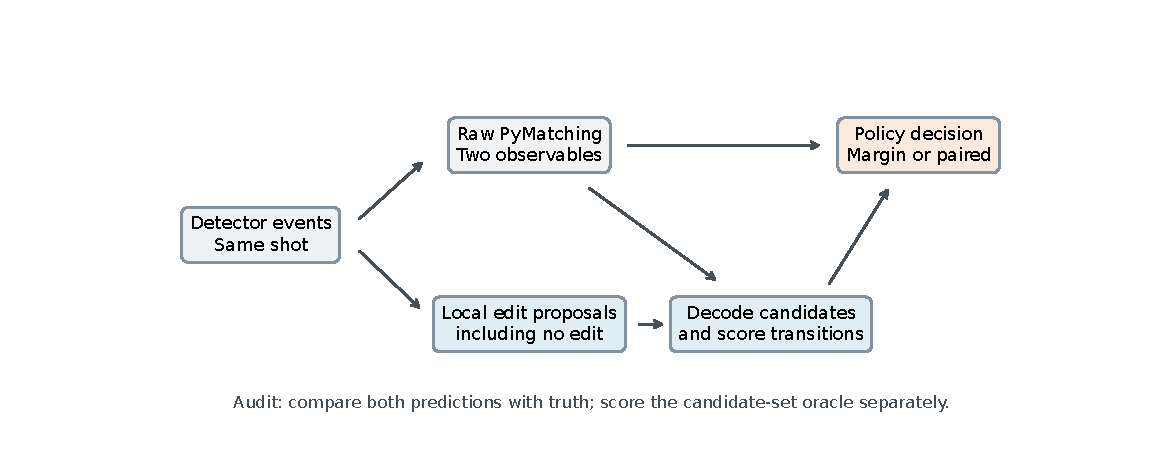
\includegraphics[width=.82\textwidth]{fig01_same_shot_method.pdf}
\caption{같은 shot에서 원본과 후보의 논리 예측을 비교하는 구조. 정답은 학습과 평가 집계에 사용한다. 추론에서 선택은 syndrome과 디코더 예측으로 수행한다.}
\label{fig:same-shot-method}
\end{figure*}

\subsection{순위, 채택, 대조군}

Top-1은 no-edit를 포함해 점수가 가장 높은 후보를 선택한다. Shot별 margin은 비영 후보와 no-edit의 점수 차이가 checkpoint별 기준에 못 미치면 원본을 유지한다. Family gate는 개발 데이터의 이득과 피해를 보고 해당 모델이 그 잡음 분포에서 수정 경로를 사용할지 결정한다. 이 gate와 shot별 기준을 따로 평가한다. 최종 독립 비교의 margin과 paired 경로는 family gate 없이 실행했다.

Paired detector는 top-1이 원본 논리 클래스의 Z bit만 바꾸고, 원본 예측을 보존하는 비영 후보도 있는 shot에 적용한다. 원본 보존 후보 중 점수가 가장 높은 것을 Z 전이 후보와 짝짓는다. 두 논리 예측 중 하나만 맞았던 개발 사례에서, Z 전이가 정답이면 양성, 원본 보존이 정답이면 음성으로 두고 L2 정규화 로지스틱 회귀를 적합했다. 특징은 두 후보의 점수 차이, 기하와 detector patch, 원본 클래스, 모델 식별자를 포함한다. 특징은 개발 평균과 표준편차로 변환하고, 표준편차의 하한은 1로 두었다. 정규화 계수는 0.01이다. Log-odds가 0 이상이면 Z 전이를 채택한다. 그 외에는 원본을 사용하며, 짝이 없는 shot에서는 기존 margin을 사용한다.

논리 gap은 같은 syndrome의 매칭 그래프 안에서 현재 클래스와 Z bit만 다른 클래스 사이의 최소 비용 차이다. 각 비용은 두 observable의 parity를 제약한 상태에서 계산했다. 원본 syndrome과 수정 syndrome 각각의 gap을 사용한 변형, detector 특징을 뺀 변형, Z 후보와 no-edit를 직접 비교하는 변형, 원본 event 통계만 이용해 Z 전환을 고르는 변형을 시험했다. 원본 기반 변형에도 적용 대상 shot을 정하려면 기존 후보 생성이 필요하다.

\section{학습과 평가 설계}

\subsection{입력 수정과 데이터 분리}

이전 실험에서는 한 데이터 family의 논리 반전 정답을 집계한 값이 입력 context의 한 채널에 포함됐다. 평가 데이터의 정답 집계가 추론 입력에 전달되는 문제를 발견한 뒤, 해당 채널을 항상 0으로 유지하고 입력 폭은 그대로 뒀다. 수정된 입력으로 거리별 모델을 다시 학습했다. 기존 d7 family gate 일부는 이전 Stage C의 결과를 본 뒤 정해졌으므로, 이후 검증에는 규칙과 모델을 먼저 고정하고 새 맵을 사용했다. 본문의 정량 결과는 수정된 입력으로 다시 학습한 checkpoint에서 얻었다.

기본 모델은 Stage A/B의 기존 데이터로 학습했다. 각 단계의 1,024 shot을 학습 717개, 검증 154개, 내부 시험 153개로 나눴다. 후보 점수 평가 경로가 학습용 구조를 재사용하는 경우에는 정답 필드를 0으로 전달했다. 후속 d7 실험에서 입력의 detector-event fraction은 약한 ZZ 개발 자료에서 얻은 0.042737로 고정했다. 교차 평가에는 기준 \(G_0\) 설정을 유지했으며, 최종 평가에서는 각 맵의 \(G_0\) context를 사용했다. 라벨은 학습 및 지표 집계에 사용했고, 평가의 후보 선택은 syndrome과 모델·디코더 출력으로 결정했다.

\begin{table*}[tb]
\centering
\caption{평가 자료와 모델 구성. Shot 수는 고정한 한 checkpoint가 받는 표본 수다.}
\label{tab:d7-1}
\small
\begin{tabularx}{\textwidth}{@{}>{\raggedright\arraybackslash}X l >{\raggedright\arraybackslash}X l@{}}
\toprule
평가 & 맵 & Shot 수 & Checkpoint \\
\midrule
입력 수정 후 거리별 재검증 & 거리별 8 & d3·d5 각각 49,152, d7 32,768 & 거리별 seed 0\textasciitilde{}7 \\
d7 잡음 변화와 전이 진단 & 8 & 강도별 43,008 & 2, 11, 54, 57 \\
d7 선택 개발과 보정 & 개발 4, 보정 2 & 맵·강도당 1,024 & seed 0\textasciitilde{}7 \\
d7 margin 독립 평가 & 788100--788123 & \(G_0\) 6,144, \(G_1\) 12,288 & seed 0\textasciitilde{}7 \\
d7 후보 생성기 비교 & 788200--788223 & \(G_1\) 12,288 & seed 0\textasciitilde{}7 \\
d7 채택 모델 독립 평가 & 788300--788323 & \(G_1\) 12,288 & seed 0\textasciitilde{}7 \\
d7 게이트 독립 평가 & 788400--788423 & \(G_1\) 12,288 & seed 0\textasciitilde{}7 \\
d7 Pauli 편향 파일럿 & 788500--788507 & 편향별 기준선 65,536, margin 16,384 & CNN seed 2 \\
d7 편향 margin 독립 평가 & 788600--788623 & \(\eta=20\), 49,152 & CNN seed 2 \\
d7 편향 채택 모델 학습 & 788700--788731 & \(\eta=20\), 65,536 & CNN seed 2 \\
d7 편향 채택 기준 선택 & 788740--788747 & \(\eta=20\), 16,384 & CNN seed 2 \\
d7 재학습 채택 모델 독립 평가 & 788800--788823 & \(\eta=20\), 49,152 & CNN seed 2 \\
\bottomrule
\end{tabularx}
\end{table*}

후속 실험에서 맵 788200--788223은 후보 생성기 비교에 사용한 뒤 채택 모델과 게이트의 개발 자료로 재사용했다. 채택 모델의 최종 평가는 맵 788300--788323, 게이트의 최종 평가는 맵 788400--788423에서 수행했다. 세 평가의 맵 집합은 서로 겹치지 않는다.

Pauli 편향 파일럿은 맵 788500--788507에서 대표 편향과 매칭 모드를 선택하는 데 사용했다. 기존 margin의 편향 독립 평가 맵 788600--788623은 후속 채택 모델의 학습·개발에 사용하지 않았다. 채택 모델의 학습, 기준 선택, 최종 평가 맵도 각각 분리했다. 편향 후속 평가는 고정 후보 CNN 하나를 사용하므로 shot 수와 모델--shot 쌍 수가 같다.

\subsection{실패 단계와 후단 디코더 비교}

같은 shot에서 원본이 틀리고 수정이 맞으면 개선, 원본이 맞고 수정이 틀리면 악화로 센다. 정확도 차이(pp)는 100에 개선 수와 악화 수의 차를 곱하고 전체 모델--shot 쌍 수로 나눈 값이다. 전체 후보 oracle은 원본 유지까지 포함해 하나라도 정답을 내면 복구 가능으로 센다. 수정 shot 고정 oracle은 기존 정책이 수정한 shot에서 비영 후보만 다시 고른다. 기존 정책이 수정하지 않은 shot에서는 원본을 유지한다. 두 oracle의 차이를 보면 수정 대상을 고르는 데 남은 회복 여지를 확인할 수 있다.

잡음 변화 평가에서는 원본과 후보의 \(D_0\) 일반 MWPM 예측을 바탕으로 \(D_0\)/\(D_1\) 교차 평가에 적용할 mask를 정했다. 후속 활성 정책 평가에서는 두 방식을 사용했다. 첫째, \(D_0\) 일반에서 정한 mask를 고정한 채 후단만 바꿨다. 둘째, 바꾼 후단의 논리 예측으로 후보 전이 특징과 점수를 다시 계산하고 mask를 선택했다. 두 방식 모두 해당 셀의 원본 PyMatching을 기준으로 비교했다. 생성 회로에서 얻은 matched DEM은 원본 syndrome의 prior이며, 수정 syndrome에서 가장 정확한 prior인지 여부는 별도의 문제다.

\subsection{최종 정책과 통계}

개발 단계에서는 강한 ZZ 맵 4개 중 3개로 head를 적합하고, 남은 맵에서 두 강도를 평가했다. 네 분할의 강한 ZZ 평균으로 정책을 골랐다. 더 복잡한 구성을 채택하려면 대조군보다 평균 정확도가 0.05 pp 이상 높고, 4개 맵 중 3개 이상에서 높아야 했다. Paired detector 대조군은 선택을 마친 뒤 개발 \(G_1\) 4맵으로 다시 적합했다. 계수와 기준은 최종 데이터 생성 전에 고정했다.

최종 평가의 주 조건은 \(G_1\)/\(D_0\) 일반 MWPM이다. Shot별 margin을 각각 원본 PyMatching과 paired detector에 비교했다. 새 맵 ID 788100\textasciitilde{}788123과 sampler seed 1794100\textasciitilde{}1794147을 사용했다. Checkpoint seed 0\textasciitilde{}7의 margin은 순서대로 1.0, 1.0, 1.25, 2.0, 0.5, 1.75, 1.0, 1.0이었다. 이 값들과 checkpoint 해시 및 표본 수를 평가 전에 고정했다. 여덟 checkpoint는 같은 shot을 공유하므로 먼저 같은 맵에서 모델을 동일 가중하고, 다음으로 24개 맵의 평균을 같은 가중치로 집계했다. 두 주 비교에 각각 양측 97.5\% Student t 구간을 적용했다. 구간이 0을 포함하면 개선 여부는 불확실로 판정했다. 약한 ZZ와 다른 디코더 셀은 보조 비교로 두고 기술 통계로 해석했다.

\subsection{후보 생성 전 게이트}

후보 탐색 전에 실행 여부를 결정하는 게이트는 첫 일반 MWPM이 반환한 비용과 라운드별 detector event 수를 입력으로 사용한다. 개발 단계에서 고정 후단이 원본 오답을 고친 경우를 \(+1\), 원본 정답을 해친 경우를 \(-1\), 그 외를 0으로 정하고, checkpoint 여덟 개에서 평균한 값을 선형 ridge 회귀의 목표로 두었다. 개발 맵 하나씩 제외하는 교차검증에서 \(\text{막은 악화}-\text{놓친 복구}\)가 가장 큰 통과 기준을 선택했다. 게이트가 막은 shot은 원본을 유지한다. 통과한 shot에는 동결한 후단을 적용한다. 후단은 후보가 출력한 대안 중 추정 정답 확률이 가장 높은 클래스의 확률에서 원본 클래스의 추정 정답 확률을 뺀다. 이 차이가 0.025를 초과할 때만 대안으로 전환한다.

강한 ZZ의 새 맵 24개에서 PyMatching 단독, 기존 후단, 게이트를 추가한 같은 후단을 비교했다. 각 맵의 512 shot을 같은 checkpoint 여덟 개에서 평가하고, 맵 평균의 차이로 95\% 신뢰구간을 계산했다. 시간은 맵마다 지정한 checkpoint 하나로 같은 batch를 세 경로에 적용해 측정했다. 한 번의 예열과 세 번의 반복에서 경로 순서를 순환했다. 첫 MWPM부터 최종 논리 예측까지 측정 범위에 포함했다. 파일 읽기와 모델·정적 구조 준비는 별도로 뒀다.

평가 전에 게이트 채택 조건 두 가지를 고정했다. 첫째, 맵별 배치 시간 절감(기존 후단의 반복 중앙값에서 게이트 경로의 반복 중앙값을 뺀 값)의 평균이 0보다 커야 한다. 둘째, PyMatching 단독 대비 게이트 경로의 정확도 차이에서 95\% 신뢰구간의 하한이 0보다 커야 한다. 두 조건을 모두 충족할 때 게이트를 채택한다.

\subsection{Pauli 편향과 채택 모델 재학습}

파일럿에서는 편향별 8개 맵의 8,192 shot을 균등 채널 DEM과 실제 편향 DEM으로 복호화하고, 일반 MWPM과 correlated matching을 비교했다. 기존 margin은 각 맵의 첫 2,048 shot에서 평가했다. 편향 DEM의 개발 오류율이 낮은 일반 MWPM을 선택하고, 조사한 가장 강한 편향인 \(\eta=20\)을 대표 조건으로 정했다. 기존 A/B 재학습 seed 2의 후보 CNN과 selector를 사용했으며, 전역 family gate를 거치지 않고 후보 경로를 직접 실행했다. CNN의 context는 파일럿의 균등 채널 기준 메타데이터와 고정 detector-event fraction을 사용했다. 저장된 selector utility 기준은 1.25였다. 최선의 비영 후보가 선택된 경우 no-edit와의 utility 차이가 이 값 이상이어야 수정을 유지했다.

기존 margin의 첫 편향 독립 평가에는 새로운 24개 맵에서 2,048 shot씩, 총 49,152 shot을 사용했다. 같은 편향 shot을 균등 채널 DEM, 편향 DEM, 편향 DEM과 margin의 결합으로 평가했다. 균등 채널 DEM에도 기존 로컬 이질성과 측정·리셋, ZZ·swap 잡음이 포함된다. 편향 DEM 대비 margin을 주 비교로 두고, 맵별 정확도 차이에 양측 95\% Student t 구간을 적용했다.

그다음 후보 CNN과 motif를 고정하고, 새로운 편향 학습 맵 32개에서 65,536 shot으로 4-class 로지스틱 채택 모델을 적합했다. 학습 target은 원본 MWPM 클래스와 정답 클래스의 XOR인 논리 전환이다. 34개 특징은 원본 matching 비용·논리 클래스, 라운드별 detector event 수, 네 논리 클래스의 상대 비용과 도달 가능 여부, 후보가 제공한 전환별 개수·첫 순위·수정 matching 비용 요약이다. 클래스별 비용은 일반 MWPM의 observable parity를 제약해 계산하고 원본 최적 비용과 일치하는지 확인했다. 특징은 학습 자료의 평균과 표준편차로 변환했고, 표준편차 하한은 \(10^{-6}\), L2 계수는 0.01로 정했다. 특징 계산에는 정답을 전달하지 않았다.

별도 개발 맵 8개의 16,384 shot에서 대안 전환 확률과 원본 유지 확률의 차이에 적용할 기준을 선택했다. 후보가 제공한 대안 중 추정 확률이 가장 높은 전환만 고려했다. 기준 후보 0, 0.01, 0.025, 0.05, 0.10, 0.20, 0.35, 0.50, 1.0 가운데 맵 평균 순이득이 가장 큰 값을 고르고, 동률이면 더 높은 기준을 선택했다. 기준 1.0은 모든 입력에서 원본을 유지한다. 선택된 기준은 0.01이며 확률 차이가 이를 초과할 때 전환했다. 같은 전환을 내는 후보 중 기존 순위의 첫 후보를 사용했고, 원본 유지에는 no-edit를 사용했다. 개발 기준 선택 후 학습 모델을 다시 적합하지 않았다.

계수와 기준값의 해시를 저장한 뒤 새로운 24개 맵의 49,152 shot에서 재학습 모델을 평가했다. 편향 DEM의 일반 MWPM 대비 새 채택 모델을 주 비교로 두고, 기존 margin과 새 모델도 같은 shot에서 비교했다. 각 독립 평가의 주 비교에는 맵 단위 양측 95\% Student t 구간을 적용하고, 하한이 0을 초과하면 추가 개선을 지지하도록 정했다. 가중치 대조와 기존 margin 대비 차이는 보조 비교로 해석했다. 이 구간은 고정 후보 CNN과 적합한 채택 모델의 새 맵 변동을 반영한다.

\section{결과}

\subsection{입력 수정 후 거리별 재검증}

수정된 입력으로 재학습한 기존 family 정책을 평가했을 때 d3의 순이득은 +2.260 pp였다. d5도 +0.022 pp였고, 관측 이득은 수정 경로를 사용한 checkpoint 하나에서 나왔다. d7에서는 여덟 모델 모두 원본을 사용했다. 따라서 d7의 구간 [0, 0]은 같은 출력을 낸 결과다. 이후 d7 실험에서는 family gate가 마스킹하던 후보 순위와 shot별 의사결정을 직접 점검했다.

\begin{table*}[tb]
\centering
\caption{수정된 입력의 거리별 독립 재검증. 구간은 d3·d5에서 97.5\%, d7에서 기술적 95\%다.}
\label{tab:d7-2}
\small
\begin{tabularx}{\textwidth}{@{}lrr>{\raggedright\arraybackslash}Xr@{}}
\toprule
거리 & Raw 정확도 (\%) & 정책 정확도 (\%) & 순이득과 구간 (pp) & 채택 \\
\midrule
d3 & 92.910 & 95.169 & +2.260 [1.688, 2.832] & 8/8 \\
d5 & 90.513 & 90.535 & +0.022 [0.004, 0.040] & 1/8 \\
d7 & 87.543 & 87.543 & 0.000 [0.000, 0.000] & 0/8 \\
\bottomrule
\end{tabularx}
\end{table*}

\subsection{d7 후보의 순위와 채택 손실}

강한 ZZ의 \(D_0\) 일반 MWPM에서 top-1은 원본 오답 10,501쌍을 고쳤고 원본 정답 25,126쌍을 해쳤다. 정확도 차이는 \ensuremath{-}8.501 pp였다. 피해가 발생한 모든 쌍에는 원본의 정답을 보존하는 다른 비영 수정이 있었다. 수정할 shot을 그대로 두고 후보만 oracle로 고르면 원본 대비 +6.107 pp였고, 모든 shot에서 후보를 다시 고르면 +11.543 pp였다. 수정 shot을 고정한 oracle이 top-1보다 추가로 맞힌 25,131쌍 가운데 25,126쌍은 원본 정답을 보존한 결과였다. 다른 후보가 원본 오답을 추가로 고친 경우는 5쌍이었다.

Shot별 margin을 적용하면 강한 ZZ의 수정률이 20.72\%에서 1.19\%로 내려갔다. 개선 948쌍과 악화 1,104쌍이 남아 순이득은 \ensuremath{-}0.091 pp였다. Family gate는 네 checkpoint 모두에서 원본을 유지했다. 약한 ZZ의 후보 oracle과 top-1 간 차이는 18.731 pp였다. 강한 ZZ에서 격차가 더 컸지만, 사전에 정한 두 강도의 top-1 순이득 차이는 \ensuremath{-}0.469 pp였고 97.5\% 구간 [\ensuremath{-}0.939, +0.065] pp에 0이 포함됐다.

\begin{figure*}[tb]
\centering
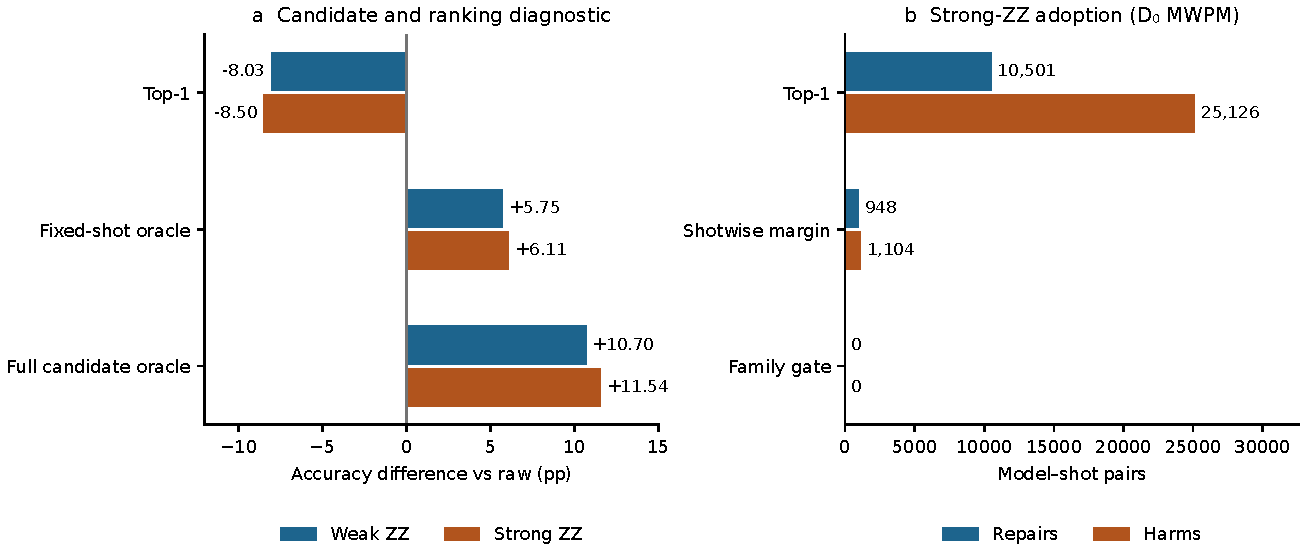
\includegraphics[width=.82\textwidth]{fig02_failure_diagnostic.pdf}
\caption{d7 후보 순위와 채택 진단. 왼쪽은 \(D_0\) 일반 MWPM에서의 원본 대비 정확도 차이다. 오른쪽은 강한 ZZ에서 각 정책이 고치거나 해친 모델--shot 쌍이다. 네 checkpoint는 각 강도의 43,008 shot을 공유한다.}
\label{fig:failure-diagnostic}
\end{figure*}

\subsection{선택 특징과 prior의 영향}

동일 syndrome의 논리 클래스별 비용은 작은 그래프의 전수 검사와 기존 d7 syndrome 44개의 독립 매칭 계산을 통해 대조했다. d7의 제약 비용 계산과 독립 매칭 계산 사이의 최대 절대 차이는 약 0.00000117이었다. 강한 ZZ 개발 교차검증에서 paired detector만 사용하면 원본 대비 \ensuremath{-}0.116 pp였다. 논리 gap을 추가한 경우 \ensuremath{-}0.095 pp로, paired 기준보다 +0.021 pp 높았다. 4맵 중 3맵에서 높았으나 평균 차이가 +0.05 pp에 못 미쳤다. 두 raw 기반 Z 전환 대조군은 강한 조건에서 전환을 적용하지 않았다. 개발 자료에서 +0.012 pp였던 기존 margin을 독립 검증할 정책으로 고정했다. 별도 보정 \(G_1\) 자료에서 같은 margin은 \ensuremath{-}0.018 pp였다.

수정 전후 syndrome의 최적 비용 차이를 점수에 추가한 선행 비교에서는 일부 mask가 바뀌었으나 수정 대상 shot을 고정했을 때 논리 예측은 같았다. 원본 클래스와 전이별로 상수 점수를 보정하는 비교에서도 수정 대상 shot을 고정하면 후보 선택이 바뀌지 않았다. 비용차 또는 전이 정보를 추가하는 것만으로 순위가 바뀌거나 개선되는지 개발 자료에서 확인할 필요가 있다.

\begin{figure*}[tb]
\centering
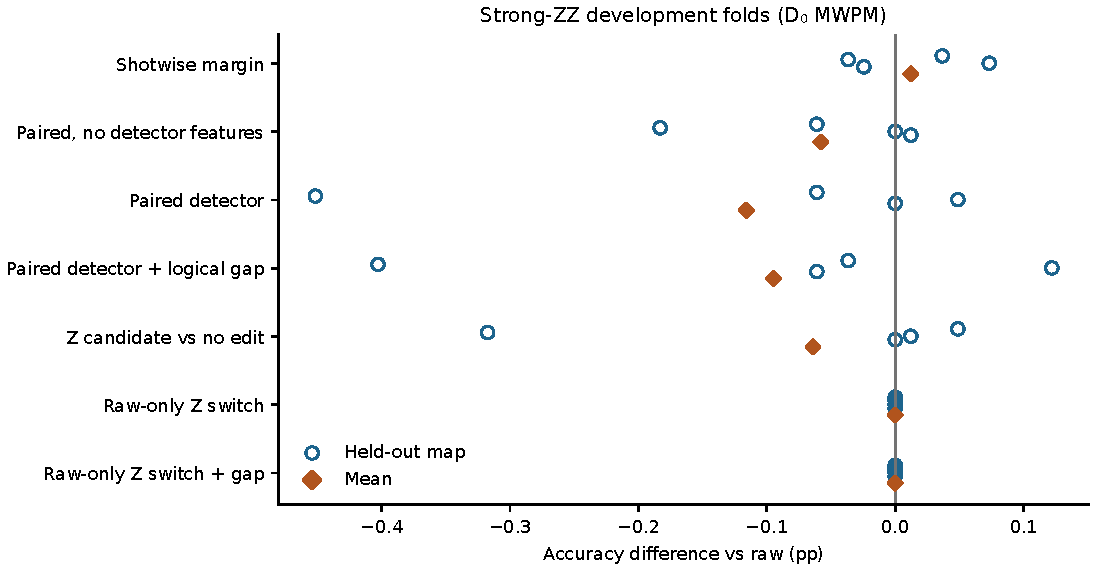
\includegraphics[width=.82\textwidth]{fig03_selector_development.pdf}
\caption{강한 ZZ의 선택기 개발 비교. 기준은 \(D_0\) 일반 MWPM이다. 각 원은 학습에서 제외한 맵의 순이득, 마름모는 네 맵의 동일 가중 평균이다.}
\label{fig:selector-development}
\end{figure*}

후단 변경의 영향은 원본과 수정의 효과로 나뉜다. 강한 ZZ 보정 자료에서 \(D_1\) correlated의 원본 정확도는 \(D_0\) 일반보다 +0.244 pp 높았다. 그러나 \(D_1\) correlated 원본을 기준으로 같은 margin mask를 적용했을 때는 \ensuremath{-}0.031 pp였고, \(D_1\) correlated로 후보 점수와 선택을 다시 계산했을 때는 +0.006 pp였다. 전체 경로에서 mask 30쌍이 바뀌었고 순정답은 1쌍 늘었다. 이 보정 자료는 2개 맵이므로, 정책의 이득이 다른 맵에서도 유지된다는 결론을 내리기 어렵다.

\subsection{24개 새 맵의 독립 평가}

사전에 지정한 강한 ZZ의 \(D_0\) 일반 MWPM에서 원본은 86.344\%, margin은 86.310\%, paired detector는 86.318\%였다. Margin은 원본 오답 139쌍을 바로잡았고 원본 정답 173쌍을 해쳤다. 원본과 paired detector에 대한 margin의 두 주 비교는 모두 97.5\% 구간에 0을 포함했다. 원본과 비교한 margin은 24맵 중 7맵에서 높고 16맵에서 낮았으며 1맵에서 같았다.

\begin{table*}[tb]
\centering
\caption{최종 평가 주 비교. \(G_1\)/\(D_0\) 일반 MWPM, 12,288 shot, 98,304 모델--shot 쌍.}
\label{tab:d7-3}
\small
\begin{tabularx}{\textwidth}{@{}lrrr>{\raggedright\arraybackslash}X@{}}
\toprule
비교 & 정확도 차이 (pp) & 97.5\% 구간 (pp) & 개선 / 악화 & 비교군 / margin 오류율 (\%) \\
\midrule
Margin vs raw & \ensuremath{-}0.035 & [\ensuremath{-}0.082, +0.013] & 139 / 173 & 13.656 / 13.690 \\
Margin vs paired & \ensuremath{-}0.008 & [\ensuremath{-}0.081, +0.065] & 283 / 291 & 13.682 / 13.690 \\
\bottomrule
\end{tabularx}
\end{table*}

같은 후보 집합의 oracle 정확도는 98.115\%로 원본보다 +11.771 pp 높았다. 독립 자료에서도 후보에 회복 여지가 있었지만 현재 margin은 이를 평균 이득으로 연결하지 못했다. \(G_1\)의 \(D_1\) correlated 원본은 \(D_0\) 일반 원본보다 +0.114 pp 높았고, 해당 correlated 원본에 margin을 더한 효과는 \ensuremath{-}0.004 pp였다. 약한 ZZ에서는 paired의 순이득이 네 디코더 셀에서 모두 양수였다. 이 결과는 사전 지정한 주 비교와 평가 강도가 다르므로 기술 통계로 보고한다.

\begin{figure*}[tb]
\centering
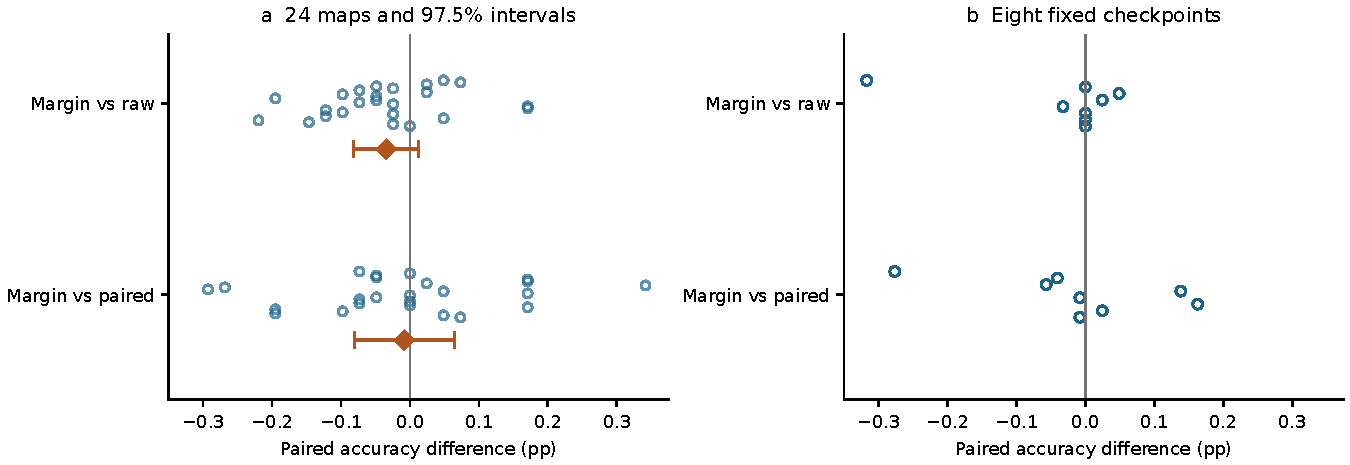
\includegraphics[width=.82\textwidth]{fig04_independent_effects.pdf}
\caption{독립 평가의 두 주 비교. 왼쪽 원은 맵별 정확도 차이, 마름모와 가로 막대는 전체 평균과 97.5\% 구간이다. 오른쪽은 고정 checkpoint별 효과다. 세로 위치를 조금씩 이동해 겹친 점을 구분했다.}
\label{fig:independent-effects}
\end{figure*}

\subsection{학습 후보 대 국소 열거}

후속 비교에서는 활성 detector의 단일 비트와 활성 detector를 포함하는 국소 비트 쌍을 신경망 없이 열거했다. 두 방법은 같은 shot과 \(D_0\) 일반 MWPM을 사용했고, 원본 유지 한 개와 고유 비영 후보 최대 32개를 허용했다. 국소 열거의 맨해튼 거리 반경은 별도 개발 맵에서 2로 정했다. 새 맵 24개에서 원본 오답에 정답 후보가 포함된 비율은 학습 후보 88.70\%, 국소 열거 77.63\%였다. 맵별 차이는 +11.07 pp(95\% 구간 [+7.63, +14.51] pp)였다. 512-shot CPU 배치에서 후보 mask 생성 시간의 중앙값은 학습 방식 1,198.8~ms, 국소 열거 96.0~ms였다. 한 shot에 나온 서로 다른 논리 클래스 수의 평균은 각각 2.47개와 2.93개였다. 학습 방식의 정답 후보 포함률 우위는 더 적은 평균 클래스 수에서 관찰됐다. 이 비교는 패턴 범위, 편집 비트 수와 순위가 함께 달라진 두 생성 방식 전체에 해당한다.

학습 후보를 유지한 뒤 원본과 대안 논리 클래스의 정답 확률을 추정하는 다항 로지스틱 채택 모델을 추가로 평가했다. 모델은 원본 syndrome의 클래스별 제약 matching 비용과 학습 후보의 논리 클래스별 개수, 첫 순위와 비용 변화를 사용했다. 개발 맵에서 채택 기준값을 0.025로 정하고 새 맵 24개에서 동결 평가했다. 변경 757쌍 중 351쌍을 고치고 401쌍을 해쳤다. 원본 대비 정확도 차이는 \ensuremath{-}0.051 pp였으며, 97.5\% 구간 [\ensuremath{-}0.199, +0.097] pp에 0이 포함됐다. 이 모델이 적용한 전환은 모두 Z 전환이었다.

\subsection{CPU 비용}

새 맵 788100의 checkpoint 2로 약한·강한 ZZ 각각 첫 256 shot에서 원본, margin, paired를 측정했다. 장치는 Intel Core i7-1165G7이었다. 각 경로에 별도 프로세스를 사용했고, PyTorch 스레드 2개와 MKL SEQUENTIAL 설정에서 한 번 워밍업한 뒤 3회 중앙값을 구했다. 메모리에 있는 syndrome에서 입력 변환, 후보 생성과 점수 계산을 거쳐 논리 예측을 얻는 구간을 측정했다. 파일 읽기와 초기 모델·DEM 구성 시간은 별도로 기록했다.

\begin{table*}[tb]
\centering
\caption{\(D_0\) 일반 MWPM의 256-shot CPU 배치 시간. 메모리는 초기 준비와 측정 중 프로세스 최대 working set이다.}
\label{tab:d7-4}
\small
\begin{tabularx}{\textwidth}{@{}lrrr>{\raggedright\arraybackslash}X@{}}
\toprule
잡음 & 원본 시간 & Margin 시간 & Paired 시간 & 최대 메모리 원본 / margin / paired (MiB) \\
\midrule
\(G_0\) & 2.373 ms & 9.173 s & 10.152 s & 268.0 / 346.6 / 350.8 \\
\(G_1\) & 1.635 ms & 12.471 s & 8.246 s & 268.6 / 350.4 / 347.7 \\
\bottomrule
\end{tabularx}
\end{table*}

원본은 배치 1회에 256개 syndrome을 매칭했다. 두 selector는 각각 257회에 8,704행을 처리했다. Selector 경로에서 matching 함수가 차지한 시간은 약 0.081\textasciitilde{}0.106초였고, 총시간의 대부분은 후보 구성과 신경망·후보 점수 계산에 쓰였다. 실행 간 변동이 커 두 selector의 속도 순위를 판단하기는 어렵다. 이번 비용은 한 장치·한 맵·한 checkpoint의 배치 측정이다.

\begin{figure*}[tb]
\centering
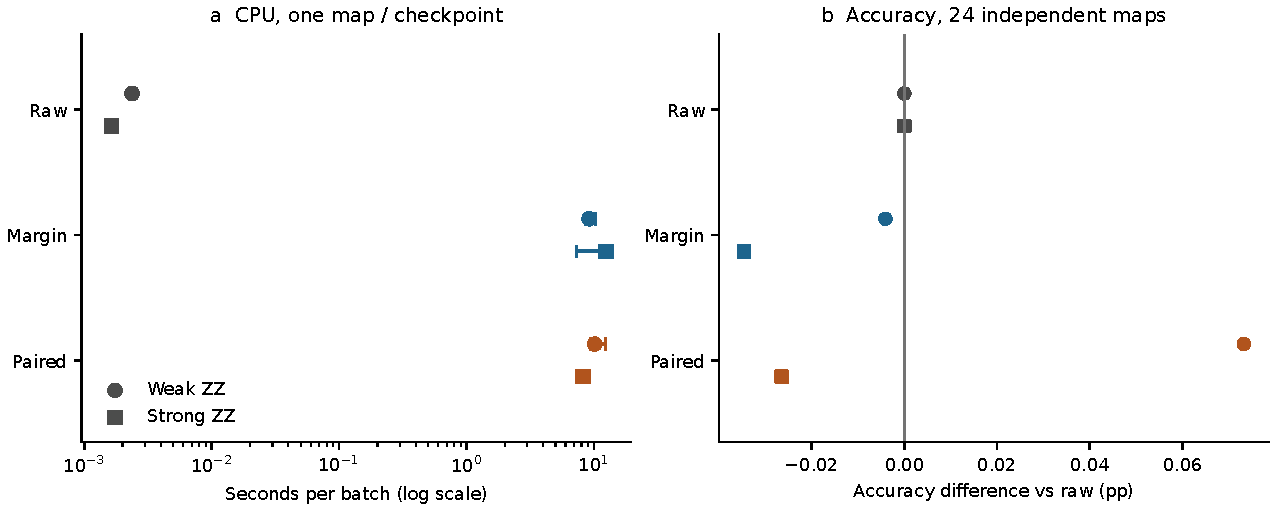
\includegraphics[width=.82\textwidth]{fig05_cost_and_accuracy.pdf}
\caption{비용과 정확도의 평가 범위. 왼쪽은 한 맵과 checkpoint에서 측정한 배치 시간 중앙값과 반복 범위다. 오른쪽은 24개 맵에서 원본 대비 얻은 정확도 차이다. 원은 약한 ZZ, 사각형은 강한 ZZ다.}
\label{fig:cost-and-accuracy}
\end{figure*}

\subsection{후보 생성 전 게이트의 정확도와 비용}

개발 맵에서 통과 목표를 90\%로 두었을 때 기존 후단의 악화 45건을 막고 복구 35건을 놓쳐, 검토한 일곱 기준 중 순효과가 가장 큰 +10건을 얻었다. 이때의 게이트를 동결하고 새 맵 24개를 평가했다. 실제 후보 탐색 실행률은 90.69\%였다. 게이트는 기존 후단의 악화 55건을 막고 복구 68건을 놓쳤다. 기존 후단 대비 순효과는 \ensuremath{-}0.013 pp(95\% 구간 [\ensuremath{-}0.079, +0.052] pp)였다.

\begin{table*}[tb]
\centering
\caption{새 맵 24개의 후보 생성 전 게이트 비교. 정확도 차이의 구간은 95\% 맵 단위 구간이다. 시간은 512-shot 배치의 반복 중앙값을 맵에서 다시 중앙값으로 집계했다.}
\label{tab:pre-gate}
\small
\begin{tabular}{@{}lrrr@{}}
\toprule
경로 & PyMatching 대비 정확도 차이 (pp) & 복구 / 악화 & 배치 시간 \\
\midrule
PyMatching 단독 & 기준 & 0 / 0 & 3.642 ms \\
기존 후단 & +0.042 [\ensuremath{-}0.144, +0.227] & 418 / 377 & 1.213 s \\
같은 후단 + 게이트 & +0.028 [\ensuremath{-}0.148, +0.205] & 350 / 322 & 1.074 s \\
\bottomrule
\end{tabular}
\end{table*}

기존 후단 대비 맵별 배치 시간 절감의 평균은 119.1 ms(95\% 구간 [97.2, 140.9] ms)였다. 24개 맵에서 모두 배치 시간이 줄었다. 실행 시간은 줄었고, 정확도 이득은 불확실했다.

% Bias sources: artifacts/eval/d7_pauli_bias/pilot/pilot_validation.json
% artifacts/eval/d7_pauli_bias/independent/validation.json
% artifacts/eval/d7_pauli_bias_adoption/validation.json
\subsection{Pauli 편향 파일럿과 첫 독립 평가}

파일럿에서 기존 margin의 편향 DEM 대비 정확도 차이는 \(\eta=0.5\)에서 +0.305 pp(95\% 구간 [+0.154, +0.456] pp), \(\eta=5\)에서 +0.128 pp([\ensuremath{-}0.069, +0.326] pp), \(\eta=20\)에서 +0.189 pp([\ensuremath{-}0.002, +0.380] pp)였다. 일반 MWPM에서 균등 채널 DEM을 편향 DEM으로 바꾼 효과는 \(\eta=5\)에서 \ensuremath{-}0.044 pp, \(\eta=20\)에서 \ensuremath{-}0.037 pp였으며 두 구간 모두 0을 포함했다. 이 자료에서 대표 편향과 매칭 모드를 고른 뒤 독립 평가를 진행했다.

첫 편향 독립 평가의 원본 논리 오류율은 14.1337\%, 기존 margin을 추가한 오류율은 14.1296\%였다(표~\ref{tab:pauli-bias-independent}). Margin은 205개를 고치고 203개를 해쳐 정답 수가 2개 늘었다. 정확도 차이 +0.0041 pp의 95\% 구간 [\ensuremath{-}0.0859, +0.0940] pp는 0을 포함했다. 같은 shot에서 균등 채널 DEM을 편향 DEM으로 바꾼 효과는 45개 복구와 45개 악화로 0.0000 pp([\ensuremath{-}0.0360, +0.0360] pp)였다. 편향을 가중치에 반영한 효과와 margin의 추가 효과 모두 이 독립 평가에서 이득을 확인하지 못했다. 원본 오답 중 후보 집합에 정답이 포함된 비율은 87.53\%였다.

\begin{table*}[tb]
\centering
\caption{Pauli 편향 \(\eta=20\)의 두 독립 평가. 각 평가는 새로운 24개 맵, 49,152 shot과 고정 후보 CNN seed 2를 사용했다. 각 집합 안의 정책은 같은 shot을 공유한다. 주 비교는 첫 평가의 margin 대 원본, 재학습 평가의 새 채택 모델 대 원본이며, 구간은 95\% 맵 단위 구간이다. 정확도 차이의 양수는 논리 오류율 감소를 뜻한다.}
\label{tab:pauli-bias-independent}
\small
\begin{tabularx}{\textwidth}{@{}>{\raggedright\arraybackslash}Xrrrr>{\raggedright\arraybackslash}X@{}}
\toprule
정책 & 오류율 (\%) & 복구 & 악화 & 원본 대비 정확도 차이 (pp) & 95\% 구간 (pp) \\
\midrule
\multicolumn{6}{@{}l}{첫 편향 독립 평가, 맵 788600--788623} \\
편향 PyMatching & 14.1337 & 기준 & 기준 & 0 & 기준 \\
기존 margin & 14.1296 & 205 & 203 & +0.0041 & [\ensuremath{-}0.0859, +0.0940] \\
\midrule
\multicolumn{6}{@{}l}{채택 모델 재학습 후 독립 평가, 맵 788800--788823} \\
편향 PyMatching & 14.4124 & 기준 & 기준 & 0 & 기준 \\
기존 margin & 14.3778 & 216 & 199 & +0.0346 & [\ensuremath{-}0.0392, +0.1084] \\
재학습 채택 모델 & 14.3941 & 199 & 190 & +0.0183 & [\ensuremath{-}0.0702, +0.1068] \\
\bottomrule
\end{tabularx}
\end{table*}

\subsection{편향 자료로 재학습한 채택 모델}

학습 자료의 target 분포는 원본 유지 56,328개, X 전환 10개, Z 전환 9,196개, Y 전환 2개였다. 개발 맵에서 기준 0.01을 선택했을 때 새 채택 모델은 80개를 복구하고 63개를 해쳐 +0.1038 pp였다. 계수와 기준을 고정한 뒤 별도의 독립 맵에서 평가한 결과, 원본 오류율 14.4124\%는 새 모델에서 14.3941\%였다. 199개 복구와 190개 악화로 정답 수 순증가는 9개였다. 원본 대비 +0.0183 pp의 95\% 구간 [\ensuremath{-}0.0702, +0.1068] pp는 0을 포함했다. 같은 shot에서 기존 margin은 +0.0346 pp였고, 새 모델 대 기존 margin의 차이는 \ensuremath{-}0.0163 pp([\ensuremath{-}0.1092, +0.0767] pp)였다. 새 모델의 추가 개선은 두 비교에서 모두 불확실했다.

새 모델과 기존 margin이 논리 예측을 바꾼 shot은 각각 389개와 415개였고, 모든 전환은 Z 전환이었다. 새 모델은 기존 margin의 악화 191개를 막았고 복구 202개를 놓쳤다. 기존 margin이 원본을 고치지 못한 경우 중 185개를 추가로 복구했으며, 원본과 기존 margin이 모두 맞은 경우 중 182개를 새로 해쳤다. 이 네 집계의 순효과는 기존 margin 대비 \ensuremath{-}8개였다. 후보 집합을 유지하고 채택 모델을 재학습해 선택 shot을 바꿨다. 이 평가에서 정확도 이득을 확인하지 못했다. 원본 오답 7,084개 중 정답 후보가 있는 경우는 6,195개, 87.45\%였다.

\section{고찰}

후보 oracle과 실제 정책의 간격은 현재 구조의 개발 우선순위를 보여 준다. 기존 top-1의 피해가 발생한 shot에서 원본을 보존할 다른 비영 후보가 있었고, 독립 자료에서도 전체 후보 집합의 oracle은 높은 정확도를 보였다. 반면 독립 주 평가에서 margin의 개선 수와 악화 수의 차이는 \ensuremath{-}34쌍이었다. 좋은 후보가 있음을 확인하는 것과 정답 없이 그 후보를 선택하는 것 사이에 간격이 남아 있다. 특히 실제 decoder를 사용할 때는 원본 정답을 해칠 위험에 비해 얼마나 많은 오답을 고쳤는지가 중요하다.

이전의 네 checkpoint로 적합한 paired head는 독립적인 강한 ZZ 맵에서 원본보다 +0.148 pp 높았다. 후속 비교에서는 여덟 checkpoint를 고정하고 새 개발 자료에서 head를 다시 학습했으며, 별개의 최종 맵에서 평가했다. 학습 자료와 모델 패널이 함께 달라졌다. Margin의 두 주 비교와 게이트의 원본 대비 비교에서 구간이 0을 포함했으므로, 각 평가에서 작은 개선과 악화가 모두 가능하다.

Pauli 편향 실험에서는 데이터 큐비트의 변경 대상 채널마다 총 오류 확률을 유지하고, 편향을 반영한 PyMatching 위에서 추가 효과를 평가했다. 기존 margin과 편향 자료로 재학습한 채택 모델의 두 독립 주 비교는 모두 95\% 구간에 0을 포함했다. 재학습은 비용·후보 요약 특징 34개를 쓰는 선형 채택 모델의 계수를 새로 적합한 것이며, 후보 CNN은 고정했다. 이 결과는 해당 특징과 모델, 고정 후보 CNN 하나에 조건부다. 입력의 공간 정보를 더 사용하는 채택 모델이나 후보 CNN 자체를 편향 자료로 학습한 경우의 성능은 이번 평가로 판단할 수 없다. 두 편향 평가의 맵 집합이 다르므로 재학습 효과를 비교할 때는 두 집합의 원본 오류율 차이 대신 같은 새 shot에서 얻은 기존 margin과 새 모델의 차이를 사용해야 한다.

재학습 평가의 원본 MWPM 오답 7,084개 중 7,077개(99.90\%)는 원본의 Z 논리 bit를 뒤집으면 정답이 되는 오류였다. 학습 target도 Z 전환 9,196개에 집중됐고 X와 Y 전환은 각각 10개와 2개였으며, 실제 두 정책의 선택은 모두 Z 전환이었다. 따라서 이번 4-class 모델 실험은 주로 어떤 shot에서 원본의 Z 논리 예측을 뒤집을지 판단하는 능력을 시험한 것으로 해석한다.

첫 편향 독립 평가에서 균등 채널 DEM과 편향 DEM의 논리 예측이 달랐던 shot은 49,152개 중 90개(0.183\%)였다. 그중 45개를 고치고 45개를 해쳤다. 이 설정에서는 가중치를 바꿔도 대부분의 논리 예측이 유지됐다. 이 낮은 변경률이 다른 잡음 채널의 기여나 매칭 경로의 안정성에서 비롯되는지는 아직 확인되지 않았다. 현재 결론은 관측한 논리 예측 변경률과 정확도 차이에 한정한다.

후보 생성 전 게이트는 기존 후단의 배치 시간을 줄였다. 같은 512-shot 배치에서 게이트 경로의 시간 중앙값은 1.074초였고, PyMatching 단독 경로는 3.642~ms였다. 후보 탐색을 건너뛴 shot은 전체의 9.31\%였다.

결과는 시뮬레이션의 Bell-pair 회로, 약한·강한 ZZ 및 데이터 큐비트 Pauli 편향 조건과 고정된 checkpoint에 해당한다. 고정 총량의 상관 잡음 유형 비교와 실제 하드웨어 평가는 별도 자료가 필요하다. 또한 현 입력은 회로 위치와 잡음에 대한 시뮬레이션 context를 포함한다. CPU 측정은 배치 처리량의 비교에 해당하며, 온라인 디코딩의 지연이나 다른 하드웨어 구현의 비용은 측정 범위 밖이다. 편향 후속 평가는 두 CPU 작업으로 병렬 실행하고 후보 재복호화 확인도 포함했으므로 그 경과 시간을 경로별 배치 지연으로 해석하지 않는다. 편향 조건의 전체 지연과 RTL 구현의 면적·지연은 추가 검증이 필요하다.

\section{결론}

동일 shot의 원본과 수정 예측을 비교한 결과, 거리 7에서 top-1의 주된 손실은 원본 정답을 해치는 논리 전환이었다. 학습 후보는 같은 예산의 국소 열거보다 원본 오답에 정답 후보를 더 자주 제공했다. 동결한 margin과 후속 채택 모델의 독립 주 평가에서 원본 대비 정확도 이득은 불확실했다. 첫 MWPM과 syndrome 정보로 후보 생성을 앞에서 거르면 기존 후단의 실행 시간을 줄일 수 있었다. 이 게이트도 원본 PyMatching 대비 정확도 이득이 확인되어야 한다는 채택 기준을 충족하지 못했다. 총 오류 확률을 유지한 데이터 큐비트 Pauli 편향 실험에서도 기존 margin의 추가 이득과 편향 자료로 새로 적합한 선형 채택 모델의 이득은 독립 평가에서 확인되지 않았다. 후보에 정답이 포함되는 비율과 실제 채택의 순이득을 함께 측정해야 함을 확인했다.

\subsection{재현성}

평가 규약, 경로별 예측과 맵별 집계, 그림·표를 생성한 코드를 저장소에 보존했다. Margin 평가에서는 384개 예측 파일과 약 1,946만 개 후보 행의 재디코딩 결과를 대조했다. 주 비교의 192개 예측 파일에서 개선·악화 수와 구간을 별도로 재계산했다. 게이트 평가에서는 새 맵 24개의 예측 파일과 반복별 시간을 검증했다. 계산에는 Stim 1.15.0과 PyMatching 2.3.1을 사용했다. 모델 패널, sampler seed, 소스 해시와 실행 명령은 집필용 근거 문서와 실행 매니페스트에서 확인할 수 있다.

첫 Pauli 편향 독립 평가에서는 24개 맵의 자료·예측과 소스·checkpoint 해시를 확인했다. 재학습 실험에서는 학습 32개·개발 8개·독립 24개 맵의 자료·특징·예측 파일을 검증했다. 재학습 모델의 정규화 평균·표준편차와 개발 기준별 이득을 재계산했고, 독립 평가의 선택 mask를 전수 재복호화했다. 정답 필드를 바꿔도 추론 예측이 같음을 확인했다. 메모리에서 변경한 단일 큐비트 확률 합을 상대 허용오차 \(10^{-12}\)로 검증했고, Stim 회로 텍스트의 유효숫자 6자리 반올림을 따로 점검했다. 첫 편향 독립 평가의 저장 회로에서 확률 합의 최대 절대 차이는 \(9.8\times10^{-9}\), 최대 상대 차이는 \(8.29\times10^{-6}\)였다. 해당 저장 회로는 상대 허용오차 \(10^{-5}\)로 검증했다. 편향 후속 코드의 구문 검사와 전체 40개 테스트를 통과했다.

\begin{thebibliography}{9}
\bibitem{fowler2012}
A. G. Fowler, M. Mariantoni, J. M. Martinis, and A. N. Cleland, “Surface codes: Towards practical large-scale quantum computation,” Physical Review A 86, 032324 (2012). \url{https://doi.org/10.1103/PhysRevA.86.032324}

\bibitem{higgott2022}
O. Higgott, “PyMatching: A Python package for decoding quantum codes with minimum-weight perfect matching,” ACM Transactions on Quantum Computing 3(3), Article 16 (2022). \url{https://doi.org/10.1145/3505637}

\bibitem{sparseblossom2025}
O. Higgott and C. Gidney, “Sparse blossom: Correcting a million errors per core second with minimum-weight matching,” Quantum 9, 1600 (2025). \url{https://doi.org/10.22331/q-2025-01-20-1600}

\bibitem{chamberland2026}
C. Chamberland, J. Olle, M. Li, S. Thornton, and I. Baratta, “Fast and accurate AI-based pre-decoders for surface codes,” arXiv:2604.12841 (2026). \url{https://arxiv.org/abs/2604.12841}

\bibitem{darmawan2024}
A. S. Darmawan, “Optimal adaptation of surface-code decoders to local noise,” arXiv:2403.08706 (2024). \url{https://arxiv.org/abs/2403.08706}

\bibitem{yoked2025}
C. Gidney, M. Newman, P. Brooks, and C. Jones, “Yoked surface codes,” Nature Communications 16, 4498 (2025). \url{https://doi.org/10.1038/s41467-025-59714-1}

\bibitem{toshio2025}
R. Toshio, K. Kishi, J. Fujisaki, H. Oshima, S. Sato, and K. Fujii, “Decoder switching: Breaking the speed-accuracy tradeoff in real-time quantum error correction,” arXiv:2510.25222 (2025). \url{https://arxiv.org/abs/2510.25222}

\bibitem{hoyt2026}
A. C. Hoyt et al., “Decoder model compatibility provides information beyond the logical gap under drifting and correlated quantum noise,” arXiv:2609.29018 (2026). \url{https://arxiv.org/abs/2609.29018}

\bibitem{stim2021}
C. Gidney, “Stim: A fast stabilizer circuit simulator,” Quantum 5, 497 (2021). \url{https://doi.org/10.22331/q-2021-07-06-497}

\end{thebibliography}

\end{document}
